\chapter{The Large Hadron Collider}

\section{scratch section to work out outline...}
First thing to do is introduce the LHC as the large hadron collider and mention where it is located.  Now I should give a brief overview of what it does.  Now I need to talk about how it does this.  That means I need to mention how the protons are accelerated.  Then I need to explain how we contain and collide them once they are accelerated.  This leads into talking about the tunnel and magnets used for steering the bunches.

\section{Introduction}
The Large Hadron Collider (LHC) is a 26.7 kilometer-long, two-ring particle accelerator and collider located on the border of France and Switzerland at the European Organization for Nuclear Research (CERN).  During normal operations the LHC maintains two counter-rotating beams of proton bunches that collide at four interaction points (IP) with up to $\sqrt{s}=14$ TeV center of mass energy and a luminosity of 10$^{34}$cm$^{-2}$s$^{-1}$.  The ALICE (Point 2), ATLAS (Point 1), CMS (Point 5), and LHC-b experiments each have a detector at one of these interaction points as scene in Figure \ref{fig:lhcips} .  The CMS and ATLAS are general-purpose detectors while LHC-b specializes in beauty quark studies.  ALICE is a heavy-ion experiment which uses $^{208}Pb-p$ or $^{208}Pb-^{208}Pb$ collisions that can also be produced by the LHC.

\begin{figure}[h]
	\centering
	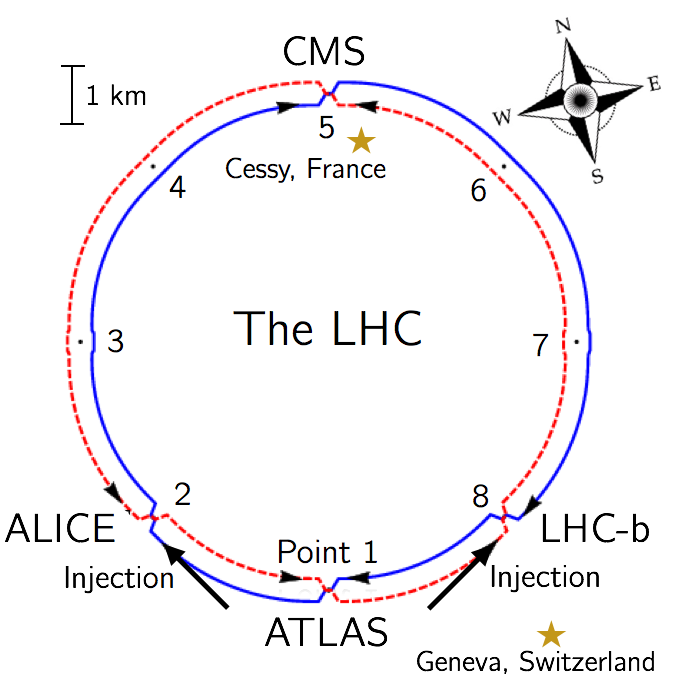
\includegraphics[width=0.7\linewidth]{Figures/LHC_IPs}
	\caption[LHC interaction points]{Interaction points of the LHC}
	\label{fig:lhcips}
\end{figure}


\section{Injection Complex}
In order to bring the protons from rest up to their target collision energy a series of accelerators is used.  The acceleration sequence begins with the injection of hydrogen gas into a duoplasmatron.  Here a bombardment of electrons ionize the hydrogen atoms while an electric field pushes them through the duoplasmatron cavity. The result is 100 keV protons being passed to a quadrapole magnet which guides them into the aperture of a linear accelerator (LINAC2).  The radio frequency (RF) cavities in LINAC2 accelerate the protons up to 50 MeV. The protons are then passed to a series of three cyclotrons before being injected into the LHC ring.  The first of these is the Proton Synchrotron Booster (PSB), which repeatedly accelerates the protons around a circular path until they reach an energy of 1.4 GeV.  The second is the Proton Synchrotron (PS) which brings the energies up to 25 GeV before sending them on to the Super Proton Synchrotron (SPS).  The SPS increases the energies to 450 GeV before finally splitting them into two beam pipes and injecting them into the LHC ring at Point 2 and Point 8.  Once in the LHC the protons are accelerated up to 6.5 TeV at which point the two counter-rotating beams can be collided to yield $\sqrt{s}=13$ center of mass energy.

The result is a packet of 100 keV protons being passed on to a quadrapole magnet which guides them into the aperture of a linear accelerator (LINAC2).  The radio frequency (RF) cavities in LINAC2 accelerate the packet of protons up to 50 MeV.  At this point the packet is split into four bunches and each bunch is sent into one of four rings in the Proton Synchrotron Booster (PSB).  The PSB increases the energy to 1.4 GeV and squeezes the protons into tighter bunches before sequentially injecting them into the single-ringed Proton Synchrotron (PS).  The protons are then passed to a series of three cyclotrons before being injected into the LHC ring.  The first of these is the Proton Synchrotron Booster (PSB), which repeatedly accelerates the protons around a circular path until they reach an energy of 1.4 GeV.  The second is the Proton Synchrotron (PS) which brings the proton energies up to 25 GeV before sending them on to the Super Proton Synchrotron (SPS).  The SPS increases the proton energies to 450 GeV before finally splitting them into two beam pipes and injecting them into the LHC ring at Point 2 and Point 8.  Once in the LHC the protons are accelerated up to 6.5 TeV at which point the two counter-rotating beams can be collided to yield $\sqrt{s}=13$ center of mass energy.

The protons are then passed to a series of three cyclotrons before being injected into the LHC.  The first of these is the Proton Synchrotron Booster (PSB), which repeatedly accelerates the protons around a 20-meter circular path until they reach an energy of 1.4 GeV.  The second is the Proton Synchrotron (PS) which brings the proton energies up to 25 GeV before sending them on to the Super Proton Synchrotron (SPS).  The SPS increases the proton energies to 450 GeV before finally splitting them into two beam pipes and injecting them into the LHC .  

  The pThe first of these is a linear accelerator (LINAC2) the accelerates protons from rest up 50 MeV.  This beam of protons then moves on the Proton Synchrotron Booster (PSB).  The PSB

\begin{figure}[h]
	\centering
	\includegraphics[width=1.0\linewidth]{Figures/LHC_sketch1}
	\caption{Layout of LHC accelerator complex.}
	\label{fig:lhcsketch}
\end{figure}


\section{Tunnel and Magnets}


\section{Luminosity} 
